\documentclass{article}
\newcommand{\mydate}{November 6, 2025}
\newcommand{\mytitle}{GP1 HW7}
\title{\textbf{\mytitle}}
\author{Jiete XUE}
\date{\mydate}
\usepackage{fancyhdr}
\pagestyle{fancy}
\fancyhf{}
\fancyhead[C]{\mytitle }
\fancyhead[R]{Jiete Xue}
\fancyhead[L]{\mydate}
\fancyfoot[C]{\thepage}
\usepackage{amsthm}
\usepackage{amsmath}
\usepackage{amssymb}
\usepackage{physics}
\usepackage{tikz}
\usepackage{float}
\usepackage{bm}

%% 右矢
%\ket{\psi}          % 输出:|ψ⟩
%\ket{\psi(t)}       % 输出:|ψ(t)⟩
%
%% 左矢
%\bra{\phi}          % 输出:⟨φ|
%
%% 期望值
%\expval{\hat{A}}    % 输出:⟨Â⟩
%\expval{\hat{A}}{\psi}  % 输出:⟨ψ|Â|ψ⟩
%
%% 对易子
%\comm{\hat{A}}{\hat{B}}  % 输出:[Â, B̂]
\newtheoremstyle{1}{}{}{}{}{\bfseries}{}{\newline}{}
\theoremstyle{1}
\newtheorem{problem}{Problem}
\usepackage{chngcntr}
\counterwithin{equation}{problem}
\newcommand{\pa}{\partial}
\newcommand{\rn}[1]{\romannumeral #1\relax}
\newcommand{\Rn}[1]{\expandafter\@slowromancap\romannumeral#1@}
\newcommand{\ii}{\mathrm{i}}
\newcommand{\ee}{\mathrm{e}}

\begin{document}
\maketitle
\begin{problem}[Angular momentum conservation]
    (1) The angular momentum is conserved
    \begin{equation}
        mv_1r_1=mv_2r_2.
    \end{equation}
    Thus, 
    \begin{equation}
        v_2=\frac{r_1}{r_2}v_1.
    \end{equation}
    (2) Work-energy theorem:
    \begin{equation}
        W=\frac{1}{2}mv_2^2-\frac{1}{2}mv_1^2=\frac{1}{2}mv_1^2\left(1-\frac{r_1^2}{r_2^2}\right).
    \end{equation}
    (3) 
    \begin{equation}
        F=m\frac{v^2}{r}=m\frac{v_1^2r_1^2}{r_2^3}.
    \end{equation}

\end{problem}
\begin{problem}[A toy of yo-yo]

    (1) Suppose the friction be $f$, acceleration be $a$, and then the angular acceleration is $\beta=\frac{a}{R}$ since no slipping.

    \begin{figure}[H]
        \centering


\tikzset{every picture/.style={line width=0.75pt}} %set default line width to 0.75pt        

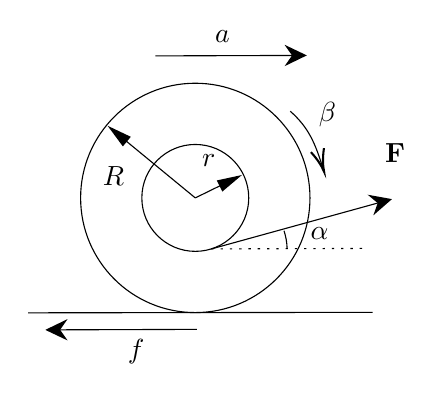
\begin{tikzpicture}[x=0.75pt,y=0.75pt,yscale=-1,xscale=1]
%uncomment if require: \path (0,300); %set diagram left start at 0, and has height of 300

%Shape: Circle [id:dp3697228457232836] 
\draw   (114,156.75) .. controls (114,142.53) and (125.53,131) .. (139.75,131) .. controls (153.97,131) and (165.5,142.53) .. (165.5,156.75) .. controls (165.5,170.97) and (153.97,182.5) .. (139.75,182.5) .. controls (125.53,182.5) and (114,170.97) .. (114,156.75) -- cycle ;
%Shape: Circle [id:dp3976287841941917] 
\draw   (84.5,156.75) .. controls (84.5,126.24) and (109.24,101.5) .. (139.75,101.5) .. controls (170.26,101.5) and (195,126.24) .. (195,156.75) .. controls (195,187.26) and (170.26,212) .. (139.75,212) .. controls (109.24,212) and (84.5,187.26) .. (84.5,156.75) -- cycle ;
%Straight Lines [id:da9010731637813859] 
\draw    (59.26,212.12) -- (225.24,211.88) ;
%Straight Lines [id:da3986031780529017] 
\draw    (147.5,181.33) -- (231.61,158.13) ;
\draw [shift={(234.5,157.33)}, rotate = 164.58] [fill={rgb, 255:red, 0; green, 0; blue, 0 }  ][line width=0.08]  [draw opacity=0] (10.72,-5.15) -- (0,0) -- (10.72,5.15) -- (7.12,0) -- cycle    ;
%Straight Lines [id:da3667641517676775] 
\draw  [dash pattern={on 0.84pt off 2.51pt}]  (147.5,181.33) -- (220.49,181.09) ;
%Shape: Arc [id:dp1565760323722598] 
\draw  [draw opacity=0] (182.5,172.6) .. controls (183.4,175.32) and (183.91,178.21) .. (183.99,181.21) -- (154,182.01) -- cycle ; \draw   (182.5,172.6) .. controls (183.4,175.32) and (183.91,178.21) .. (183.99,181.21) ;  
%Straight Lines [id:da0960842730297835] 
\draw    (70.5,220.32) -- (140.49,220.09) ;
\draw [shift={(67.5,220.33)}, rotate = 359.81] [fill={rgb, 255:red, 0; green, 0; blue, 0 }  ][line width=0.08]  [draw opacity=0] (10.72,-5.15) -- (0,0) -- (10.72,5.15) -- (7.12,0) -- cycle    ;
%Straight Lines [id:da6069453426064472] 
\draw    (139.75,156.75) -- (160.42,146.61) ;
\draw [shift={(162.21,145.73)}, rotate = 153.86] [fill={rgb, 255:red, 0; green, 0; blue, 0 }  ][line width=0.08]  [draw opacity=0] (12,-3) -- (0,0) -- (12,3) -- cycle    ;
%Straight Lines [id:da47543815734711725] 
\draw    (99.04,123.27) -- (139.75,156.75) ;
\draw [shift={(97.5,122)}, rotate = 39.44] [fill={rgb, 255:red, 0; green, 0; blue, 0 }  ][line width=0.08]  [draw opacity=0] (12,-3) -- (0,0) -- (12,3) -- cycle    ;
%Straight Lines [id:da44467489416814365] 
\draw    (120.5,88.33) -- (190.49,88.1) ;
\draw [shift={(193.49,88.09)}, rotate = 179.81] [fill={rgb, 255:red, 0; green, 0; blue, 0 }  ][line width=0.08]  [draw opacity=0] (10.72,-5.15) -- (0,0) -- (10.72,5.15) -- (7.12,0) -- cycle    ;
%Curve Lines [id:da9256303565237991] 
\draw    (185.5,115) .. controls (194.39,122.81) and (197.52,130.46) .. (201.27,142.46) ;
\draw [shift={(201.81,144.18)}, rotate = 252.9] [color={rgb, 255:red, 0; green, 0; blue, 0 }  ][line width=0.75]    (10.93,-3.29) .. controls (6.95,-1.4) and (3.31,-0.3) .. (0,0) .. controls (3.31,0.3) and (6.95,1.4) .. (10.93,3.29)   ;

% Text Node
\draw (230,129.4) node [anchor=north west][inner sep=0.75pt]    {$\mathbf{F}$};
% Text Node
\draw (194,170) node [anchor=north west][inner sep=0.75pt]    {$\alpha $};
% Text Node
\draw (105.99,223.61) node [anchor=north west][inner sep=0.75pt]    {$f$};
% Text Node
\draw (94,140.4) node [anchor=north west][inner sep=0.75pt]    {$R$};
% Text Node
\draw (141.75,134.4) node [anchor=north west][inner sep=0.75pt]    {$r$};
% Text Node
\draw (148,75) node [anchor=north west][inner sep=0.75pt]    {$a$};
% Text Node
\draw (198,109.4) node [anchor=north west][inner sep=0.75pt]    {$\beta $};


\end{tikzpicture}
\caption{Toy of yo-yo}
    \end{figure}
We have
    \begin{equation}
        F\cos \alpha-f=ma,
    \end{equation}
    \begin{equation}
        fR-Fr=I\frac{a}{R}.
    \end{equation}
So,
\begin{equation}
    a=F\frac{R\cos \alpha-r}{mR+I/R}.
\end{equation}
(2) When $F>\frac{mg}{\sin \alpha}$, the yo-yo can be lift off the table.
\end{problem}
\begin{problem}[Bounce back]
    Suppose the force in horizontal given by table during the collision is $F$. Then,
    \begin{equation}
        F=ma,
    \end{equation}
    \begin{equation}
        F(h-r)=\frac{2}{5}mr^2\beta.
    \end{equation}
    Since it is still a pure rolling,
    \begin{equation}
        r\beta=a.
    \end{equation}
    Therefore,
    \begin{equation}
        \frac{h}{r}=\frac{7}{5}.
    \end{equation}
\end{problem}
\begin{problem}[Euler equations]
    (1) 
    \begin{equation}
        \frac{\dd \mathbf{L}}{\dd t}=\frac{\tilde{\dd}\mathbf{L}}{\dd{t}}+\bm{\omega}\times\mathbf{L}=0.
    \end{equation}
    So the angular momentum is conserved.
    \newline
    (2) 
    \begin{equation}
        \mathbf{L}=\mathbf{I}\cdot\bm{\omega}.
    \end{equation}
    \begin{equation}
        T=\frac{1}{2}\bm{\omega}\cdot\mathbf{L}.
    \end{equation}
    Since $\bm{I}$ is a symmetric second order tensor,
    \begin{equation}
        \frac{\dd{\bm{\omega}}}{\dd{t}}\cdot \bm{I}\cdot\bm{\omega}=\bm{\omega}\cdot \bm{I}\cdot\frac{\dd{\bm{\omega}}}{\dd{t}}
    \end{equation}
    \begin{equation}
        2\frac{\dd T}{\dd t}=\frac{\dd{\bm{\omega}}}{\dd{t}}\cdot\bm{L}+\bm{\omega}\cdot\frac{\dd\mathbf{L}}{\dd{t}}=2\bm{\omega}\cdot\frac{\dd\mathbf{L}}{\dd{t}}=0.
    \end{equation}
    So the kinetic energy of rotation is a constant.
\end{problem}
\end{document}